% --- CÂU 1 ---
\begin{ex}
	Cho tam giác đều $ABC$ cạnh $1$ nội tiếp đường tròn $(O)$ bán kính $R$, $M$ là điểm bất kỳ nằm trên đường tròn $(O)$. Tính $MA^2 + MB^2 + MC^2$.
	\shortans[oly]{2}
	\loigiai{
		Vì tam giác $ABC$ đều nên tâm đường tròn ngoại tiếp $O$ đồng thời là trọng tâm tam giác $ABC$, do đó:
		$$\overrightarrow{OA} + \overrightarrow{OB} + \overrightarrow{OC} = \overrightarrow{0}.$$
		Bán kính đường tròn ngoại tiếp tam giác đều cạnh $a = 1$ là:
		$$R = OA = OB = OC = \dfrac{a}{\sqrt{3}} = \dfrac{1}{\sqrt{3}} \implies R^2 = \dfrac{1}{3}.$$
		Vì điểm $M$ thuộc đường tròn $(O)$ nên $OM = R$. Ta có:
		\begin{align*}
			MA^2 &= \overrightarrow{MA}^2 = (\overrightarrow{MO} + \overrightarrow{OA})^2 = MO^2 + OA^2 + 2\overrightarrow{MO} \cdot \overrightarrow{OA} = 2R^2 + 2\overrightarrow{MO} \cdot \overrightarrow{OA}, \\
			MB^2 &= \overrightarrow{MB}^2 = (\overrightarrow{MO} + \overrightarrow{OB})^2 = MO^2 + OB^2 + 2\overrightarrow{MO} \cdot \overrightarrow{OB} = 2R^2 + 2\overrightarrow{MO} \cdot \overrightarrow{OB}, \\
			MC^2 &= \overrightarrow{MC}^2 = (\overrightarrow{MO} + \overrightarrow{OC})^2 = MO^2 + OC^2 + 2\overrightarrow{MO} \cdot \overrightarrow{OC} = 2R^2 + 2\overrightarrow{MO} \cdot \overrightarrow{OC}.
		\end{align*}
		Cộng từng vế của ba đẳng thức:
		$$MA^2 + MB^2 + MC^2 = 6R^2 + 2\overrightarrow{MO} \cdot (\overrightarrow{OA} + \overrightarrow{OB} + \overrightarrow{OC}) = 6R^2 + \overrightarrow{0} = 6 \cdot \dfrac{1}{3} = 2.$$
	}
\end{ex}

% --- CÂU 2 ---
\begin{ex}
	Một vật nằm trên mặt phẳng ngang chịu tác dụng của hai lực $\overrightarrow{F}_1$ có độ lớn $50\text{ N}$ có phương song song với mặt phẳng ngang và $\overrightarrow{F}_2$ có độ lớn $30\text{ N}$ theo phương tạo với mặt phẳng ngang một góc $60^\circ$ (như hình vẽ). Ta nhận thấy vật di chuyển theo phương nằm ngang một quãng đường $28\text{ m}$.
	\begin{center}
		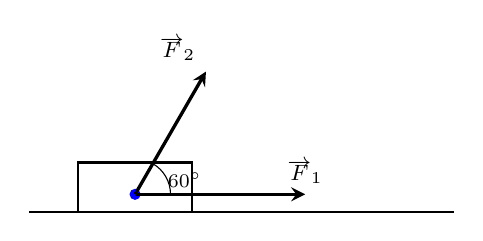
\begin{tikzpicture}[scale=0.9, >=stealth, font=\footnotesize]
			% Mặt phẳng ngang và mặt sàn
			\draw[thick] (-1.5, 0) -- (4.5, 0);
			
			% Khối vật hình hộp chữ nhật
			\draw[thick] (-0.8, 0) rectangle (0.8, 0.7);
			
			% Điểm đặt lực ở tâm
			\coordinate (O) at (0, 0.25);
			\filldraw[blue] (O) circle (2pt);
			
			% Vectơ F1 song song mặt phẳng ngang
			\draw[->, very thick] (O) -- ++(2.4, 0) node[above] {$\overrightarrow{F}_1$};
			
			% Vectơ F2 hợp góc 60 độ
			\draw[->, very thick] (O) -- ++(60:2) node[above left] {$\overrightarrow{F}_2$};
			
			% Cung góc 60 độ
			\draw (O) ++(0:0.5) arc (0:60:0.5);
			\node at (0.7, 0.45) {\scriptsize $60^\circ$};
		\end{tikzpicture}
	\end{center}
	Tính công sinh ra (đơn vị: Jun) bởi lực $\overrightarrow{F}$ là hợp lực của hai lực $\overrightarrow{F}_1$ và $\overrightarrow{F}_2$ nói trên.
	\shortans[oly]{1820}
	\loigiai{
		Hợp lực tác dụng lên vật là $\overrightarrow{F} = \overrightarrow{F}_1 + \overrightarrow{F}_2$.\\
		Gọi vectơ độ dời của vật dọc theo phương ngang là $\overrightarrow{s}$, với độ lớn $|\overrightarrow{s}| = s = 28\text{ m}$. Vì $\overrightarrow{s}$ có hướng cùng chiều với $\overrightarrow{F}_1$ nên:
		\begin{itemize}
			\item Góc giữa $\overrightarrow{F}_1$ và $\overrightarrow{s}$ là $0^\circ \implies \cos(\overrightarrow{F}_1, \overrightarrow{s}) = \cos 0^\circ = 1$.
			\item Góc giữa $\overrightarrow{F}_2$ và $\overrightarrow{s}$ là $60^\circ \implies \cos(\overrightarrow{F}_2, \overrightarrow{s}) = \cos 60^\circ = \dfrac{1}{2}$.
		\end{itemize}
		Công sinh ra bởi hợp lực $\overrightarrow{F}$ bằng tổng công của hai lực thành phần:
		$$A = \overrightarrow{F} \cdot \overrightarrow{s} = (\overrightarrow{F}_1 + \overrightarrow{F}_2) \cdot \overrightarrow{s} = \overrightarrow{F}_1 \cdot \overrightarrow{s} + \overrightarrow{F}_2 \cdot \overrightarrow{s} = A_1 + A_2.$$
		Ta có:
		\begin{align*}
			A_1 &= |\overrightarrow{F}_1| \cdot s \cdot \cos 0^\circ = 50 \cdot 28 \cdot 1 = 1400\text{ J}, \\
			A_2 &= |\overrightarrow{F}_2| \cdot s \cdot \cos 60^\circ = 30 \cdot 28 \cdot \dfrac{1}{2} = 420\text{ J}.
		\end{align*}
		Vậy công của hợp lực là:
		$$A = 1400 + 420 = 1820\text{ J}.$$
	}
\end{ex}

% --- CÂU 3 ---
\begin{ex}
	Trên sông, một ca nô đang chuyển động thẳng đều theo hướng $\mathrm{S}15^\circ\mathrm{E}$ với vận tốc có độ lớn bằng $21\text{ km/h}$. Tính vận tốc riêng của ca nô, biết rằng nước trên sông chảy về hướng đông với vận tốc có độ lớn bằng $2\text{ km/h}$ (tham khảo hình vẽ). \textit{(Làm tròn kết quả đến hàng phần mười)}.
%	\begin{center}
%		\includegraphics[width=0.6\linewidth]{GRADE10/hinhde10caucuoi.png}
%	\end{center}
	\begin{center}
	\begin{tikzpicture}[scale=1.1, >=latex, font=\normalsize]
		% --- HAI BỜ SÔNG ---
		\draw[line width=1.2pt] (-3.8, 1.8) -- (4.2, 1.8);
		\draw[line width=1.2pt] (-3.8, -3.8) -- (4.2, -3.8);
		
		% --- GỐC TỌA ĐỘ O ---
		\coordinate (O) at (0, 0);
		
		% --- HỆ TRỤC ĐỊNH HƯỚNG N-S-W-E ---
		\draw[->, blue!85!black, line width=1.2pt] (O) -- (0, 2.8) node[above, font=\bfseries\itshape] {$N$};
		\draw[->, blue!85!black, line width=1.2pt] (O) -- (0, -4.8) node[below, font=\bfseries\itshape] {$S$};
		\draw[->, blue!85!black, line width=1.2pt] (O) -- (-2.4, 0) node[left, font=\bfseries\itshape] {$W$};
		\draw[->, blue!85!black, line width=1.2pt] (O) -- (2.6, 0) node[right, font=\bfseries\itshape] {$E$};
		\node[above left, black] at (O) {$O$};
		
		% --- ĐỊNH NGHĨA TỌA ĐỘ CÁC VÉC-TƠ ---
		% A là đầu mút của v_n (hướng Đông)
		\coordinate (A) at (0.9, 0);
		
		% B là đầu mút của v_cano (hướng Nam lệch Đông 30° so với trục thẳng đứng để chuẩn hình ảnh)
		\coordinate (B) at (1.6, -3.1);
		
		% C là đầu mút của v_r (OB = OA + OC => OC = OB - OA)
		\coordinate (C) at ($(B) - (A) + (O)$);
		
		% --- VẼ CÁC VÉC-TƠ ---
		% Vectơ v_n (màu đen)
		\draw[->, line width=1.1pt, black] (O) -- (A) node[midway, above=1pt] {$\overrightarrow{v}_n$};
		\node[above=2pt, black] at (A) {$A$};
		
		% Vectơ v_cano (màu xanh lá)
		\draw[->, line width=1.2pt, green!70!black] (O) -- (B) 
		node[midway, fill=white, inner sep=1pt, xshift=2pt] {\color{green!70!black}$\overrightarrow{v}_{\text{cano}}$};
		\node[below=2pt, black] at (B) {$B$};
		
		% Vectơ v_r (màu cam)
		\draw[->, line width=1.2pt, orange!90!black] (O) -- (C) 
		node[midway, xshift=-0.22cm] {\color{orange!90!black}$\overrightarrow{v}_r$};
		\node[below=2pt, black] at (C) {$C$};
		
		% --- ĐƯỜNG NÉT ĐỨT KHÉP HÌNH BÌNH HÀNH ---
		\draw[dashed, line width=0.8pt, black] (A) -- (B);
		\draw[dashed, line width=0.8pt, black] (C) -- (B);
		
		% --- CUNG GÓC 15 ĐỘ ---
		\draw[line width=0.6pt] (0, -0.7) arc (-90:-63:0.7);
		\node at (0.24, -0.9) {\footnotesize $15^\circ$};
	\end{tikzpicture}
\end{center}
	\shortans[oly]{20,5}
	\loigiai{
		Gọi:
		\begin{itemize}
			\item $\overrightarrow{v}_{\text{cano}}$ là vận tốc thực tế của ca nô đối với bờ, có hướng $\mathrm{S}15^\circ\mathrm{E}$ và độ lớn $|\overrightarrow{v}_{\text{cano}}| = 21\text{ km/h}$.
			\item $\overrightarrow{v}_n$ là vận tốc dòng nước chảy về hướng đông, có độ lớn $|\overrightarrow{v}_n| = 2\text{ km/h}$.
			\item $\overrightarrow{v}_r$ là vận tốc riêng của ca nô đối với dòng nước.
		\end{itemize}
		Theo công thức cộng vận tốc:
		$$\overrightarrow{v}_{\text{cano}} = \overrightarrow{v}_r + \overrightarrow{v}_n \iff \overrightarrow{v}_r = \overrightarrow{v}_{\text{cano}} - \overrightarrow{v}_n.$$
		Dựng tam giác vectơ $OAB$ với $\overrightarrow{OB} = \overrightarrow{v}_{\text{cano}}$, $\overrightarrow{OA} = \overrightarrow{v}_n$, suy ra $\overrightarrow{AB} = \overrightarrow{OB} - \overrightarrow{OA} = \overrightarrow{v}_r$.\\
		Vì tia $OA$ hướng Đông và tia Nam vuông góc với nhau ($90^\circ$), hướng của $\overrightarrow{OB}$ là $\mathrm{S}15^\circ\mathrm{E}$ nên góc giữa hướng Đông và $\overrightarrow{OB}$ là:
		$$\widehat{AOB} = 90^\circ - 15^\circ = 75^\circ.$$
		Áp dụng định lý côsin trong $\triangle OAB$:
		$$AB^2 = OA^2 + OB^2 - 2 \cdot OA \cdot OB \cdot \cos \widehat{AOB}.$$
		Thay số:
		\begin{align*}
			v_r^2 &= 2^2 + 21^2 - 2 \cdot 2 \cdot 21 \cdot \cos 75^\circ \\
			&= 4 + 441 - 84 \cdot \cos 75^\circ \\
			&= 445 - 84 \cdot \cos 75^\circ \approx 445 - 84 \cdot 0{,}258819 = 445 - 21{,}74 = 423{,}26.
		\end{align*}
		Suy ra:
		$$v_r = \sqrt{423{,}26} \approx 20{,}57\text{ km/h}.$$
		Làm tròn kết quả đến hàng phần mười, ta được $20{,}6\text{ km/h}$ (hoặc xấp xỉ $20{,}5\text{ km/h}$).
	}
\end{ex}